\renewcommand{\thefootnote}{\arabic{footnote}}

\section{Data}

\begin{figure}[tb]
  \centerline{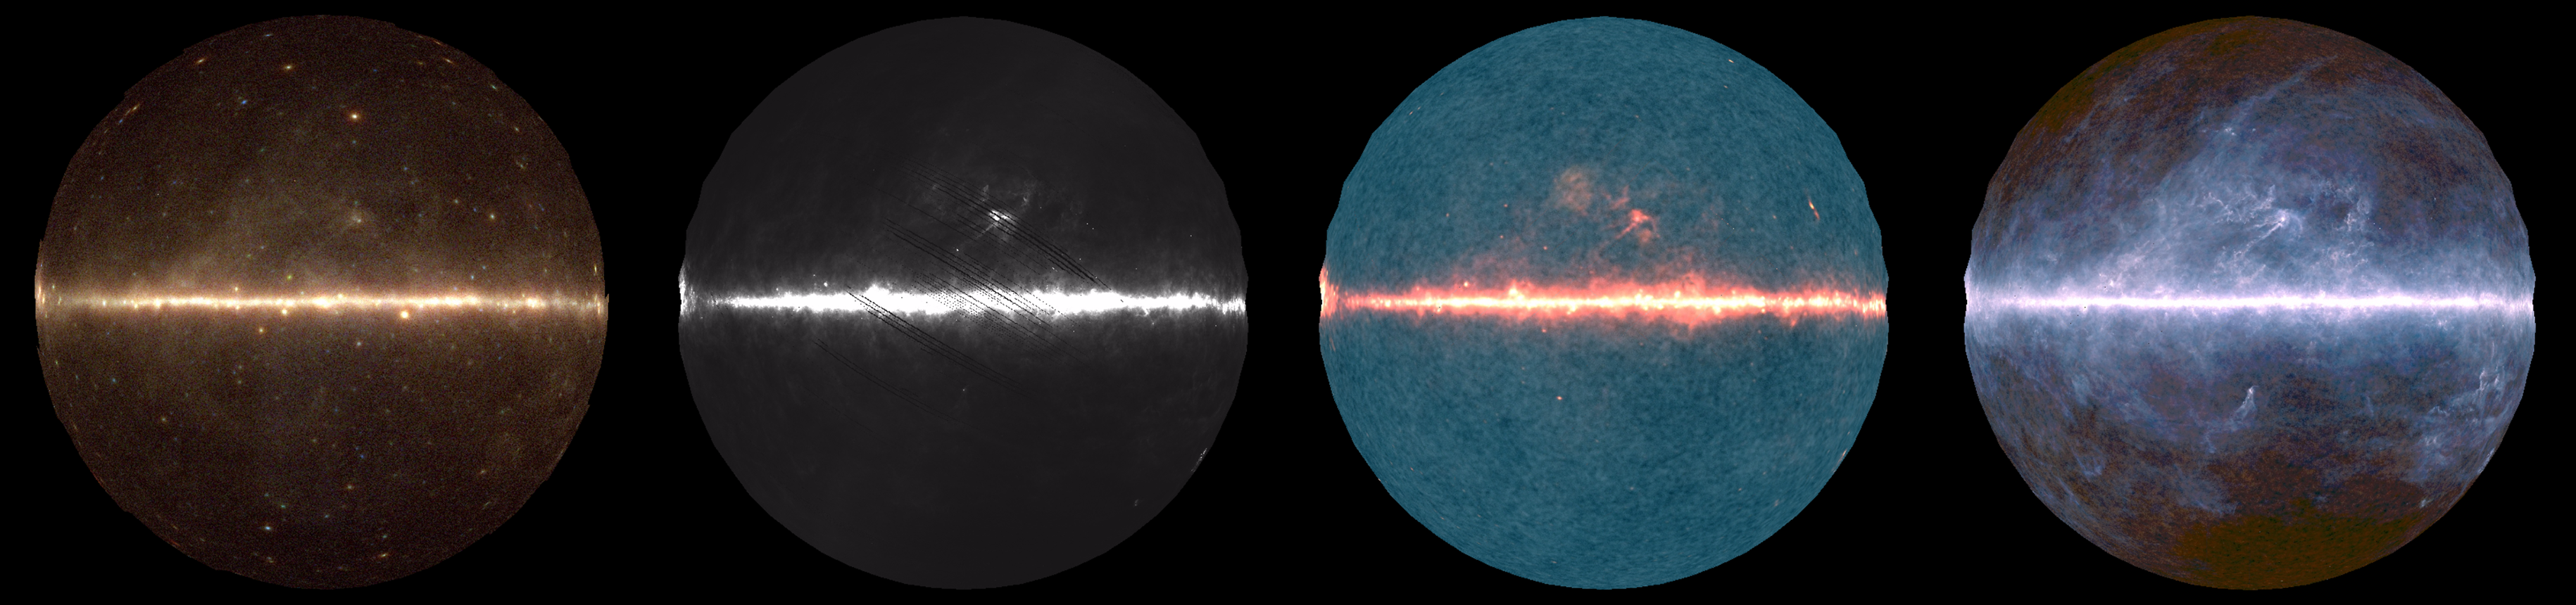
\includegraphics[width=\textwidth]{figures/four_images}}
  \caption{Survey images (left to right): Fermi color, AKARI 90um, Planck LFI, Planck HFI. Images centered on the Galactic Center, FOV 180 degrees.}
  \label{fig:four_images}
\end{figure}

\begin{figure}[tb]
  \centerline{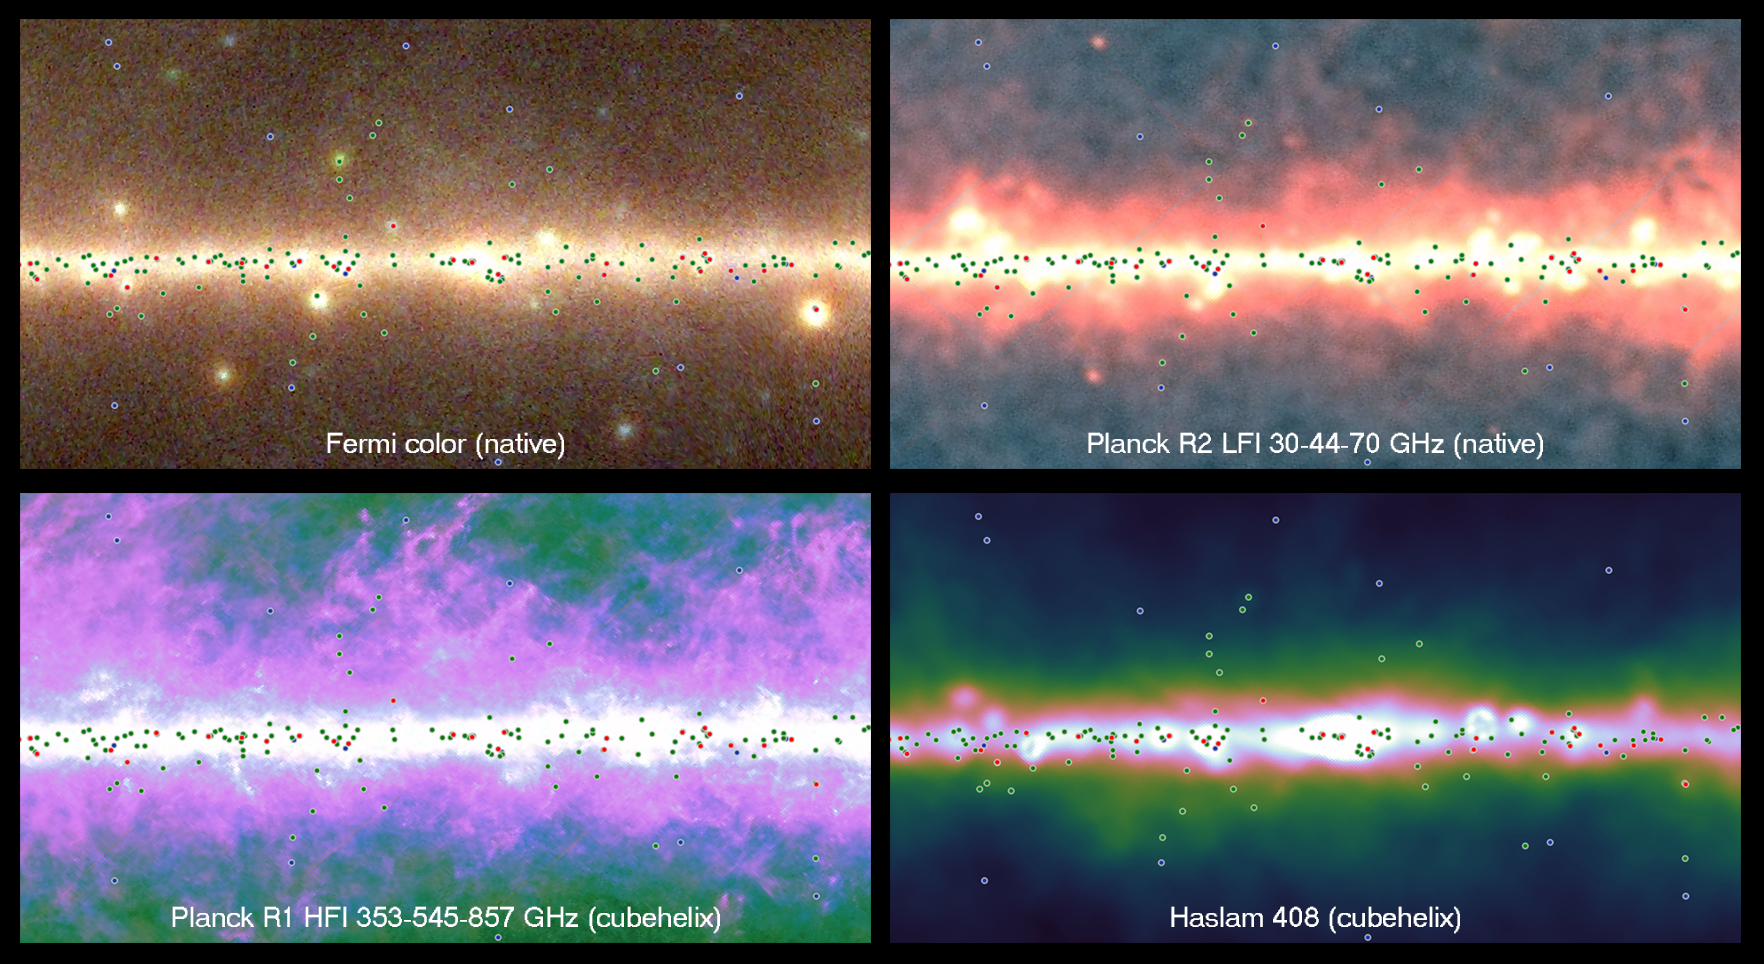
\includegraphics[width=\textwidth]{figures/inner_galaxy_region}}
  \caption{The inner galaxy in various survey images and color maps, FOV 45 degrees.}
\end{figure}

\begin{figure}[tb]
  \centerline{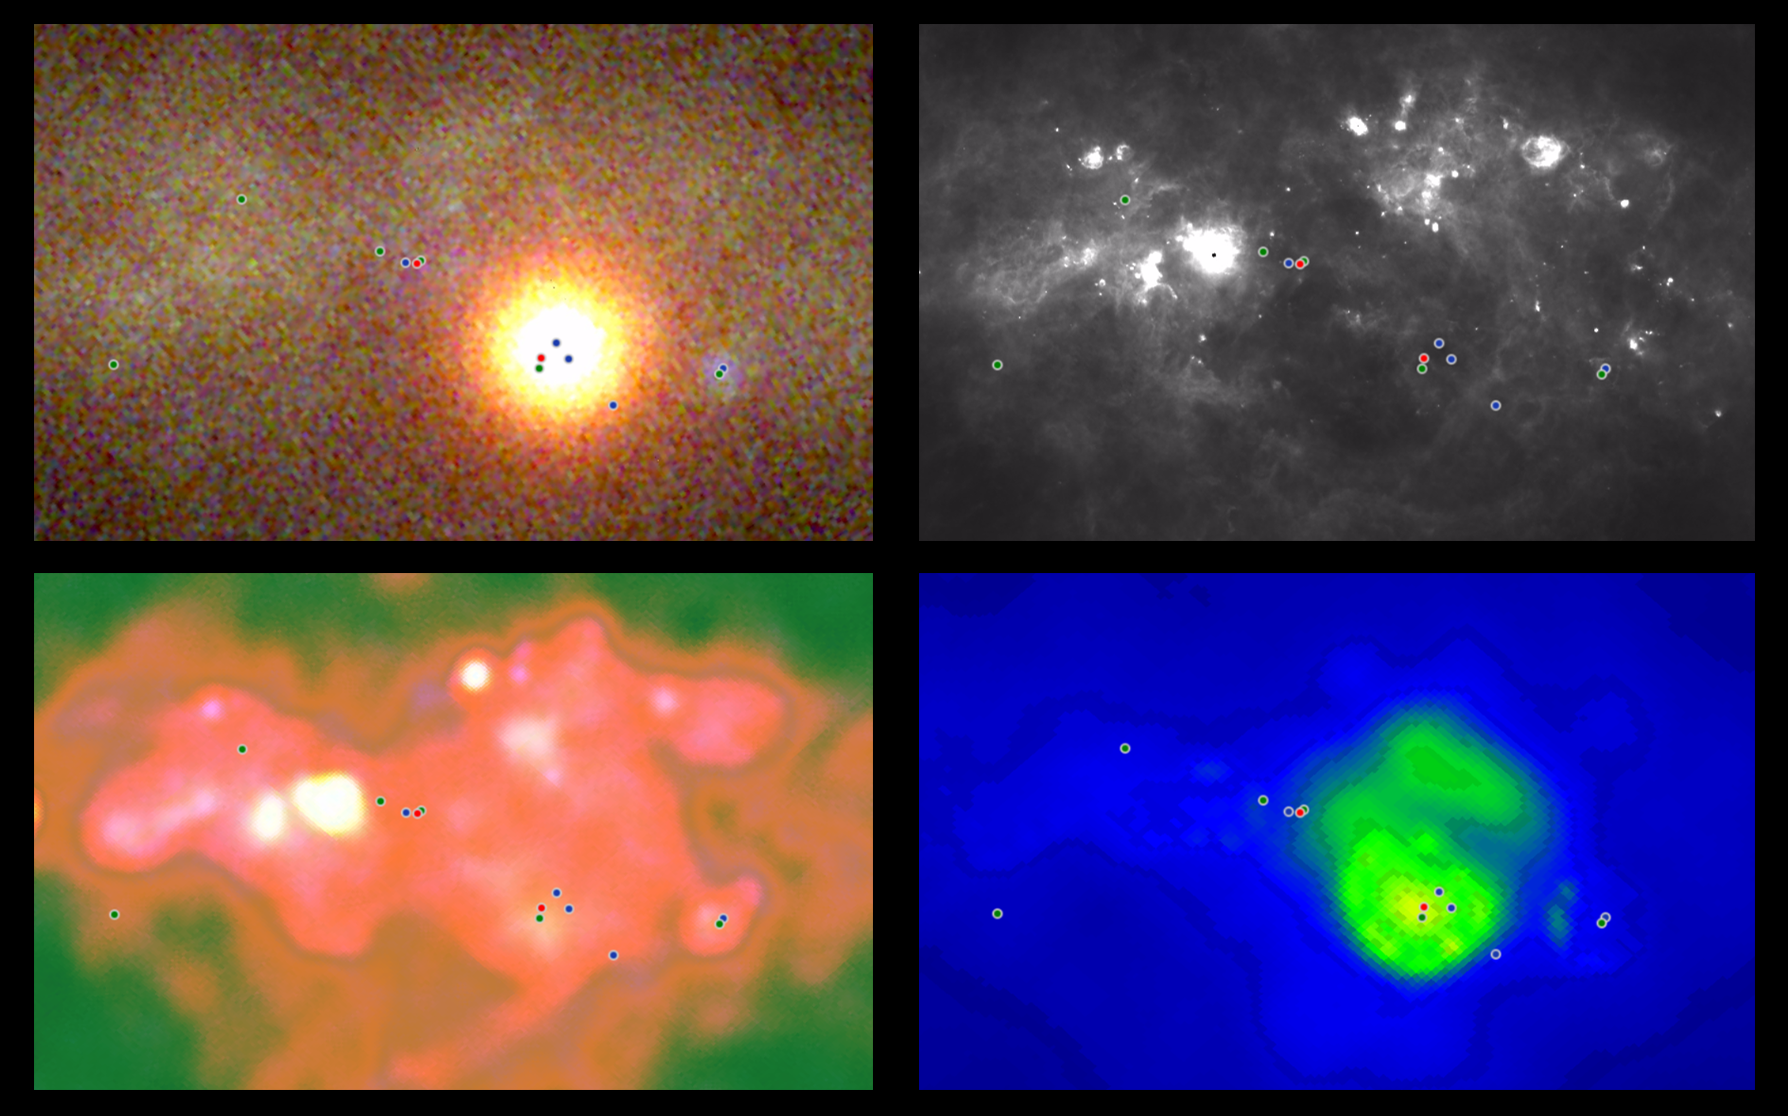
\includegraphics[width=\textwidth]{figures/vela_region}}
  \caption{The Vela Region in various survey images and color maps, FOV 20 degrees.}
  \label{fig:vela_region}
\end{figure}


% \begin{figure}[tb]
%   \centerline{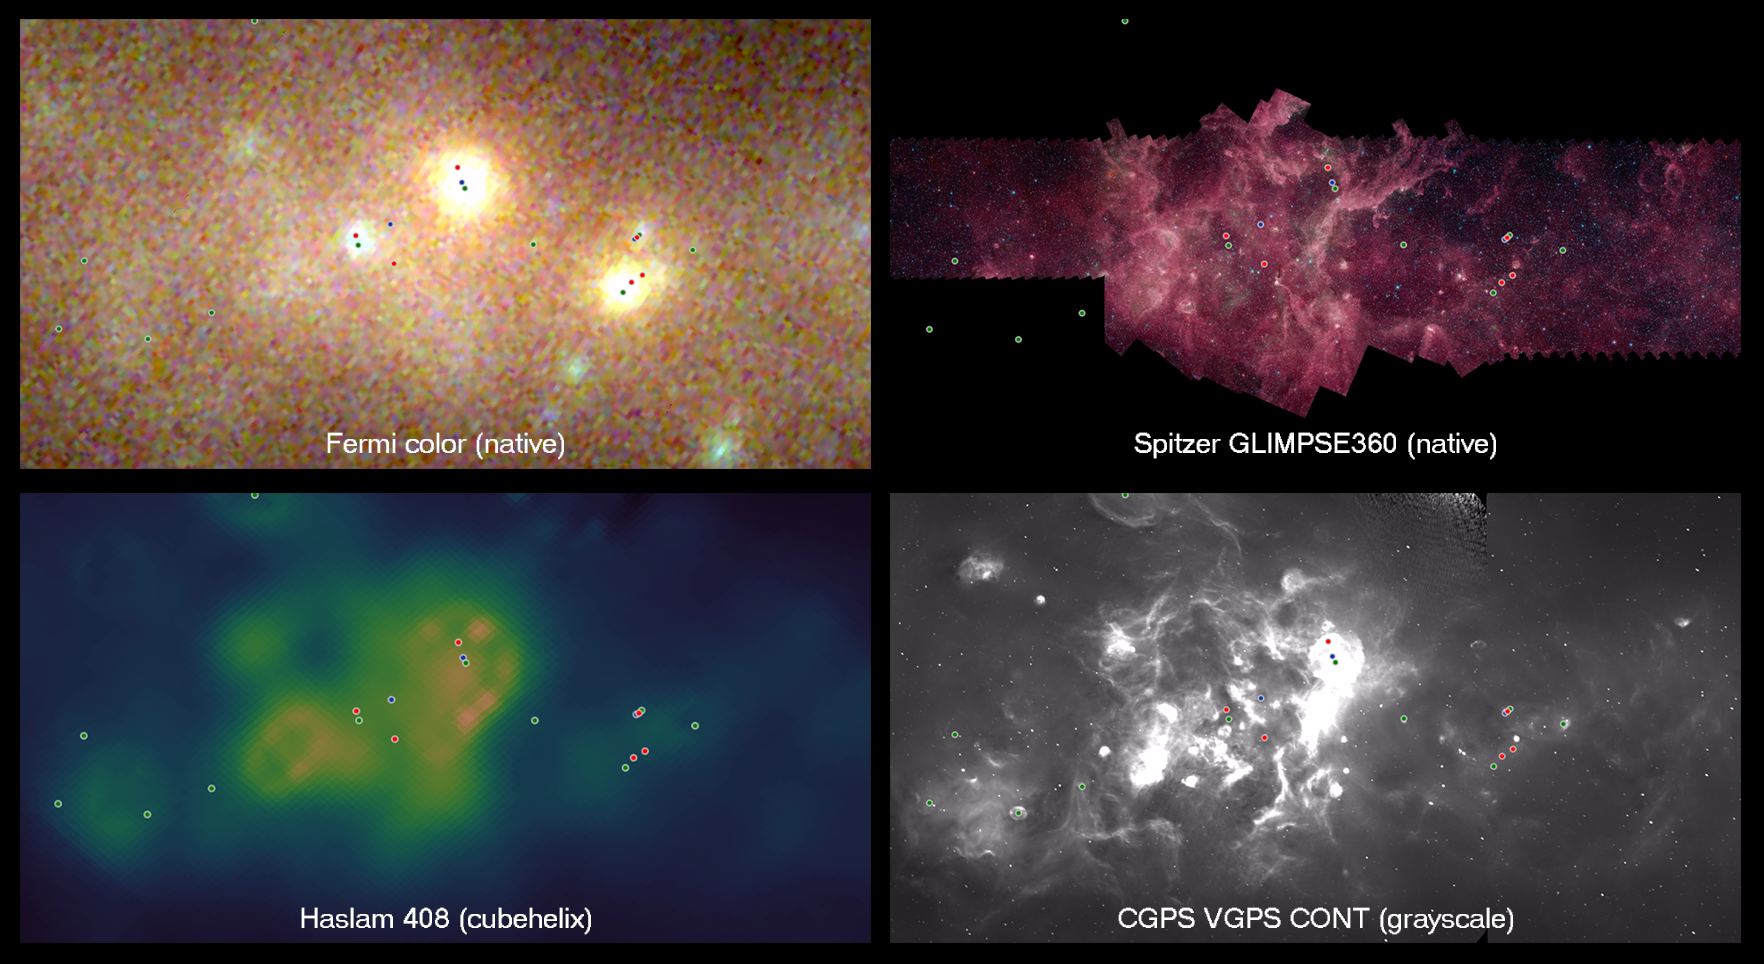
\includegraphics[width=\textwidth]{figures/cygnus_region}}
%   \caption{The Cygnus Region in various survey images and color maps, FOV 20 degrees.}
% \end{figure}
%
% \begin{figure}[tb]
%   \centerline{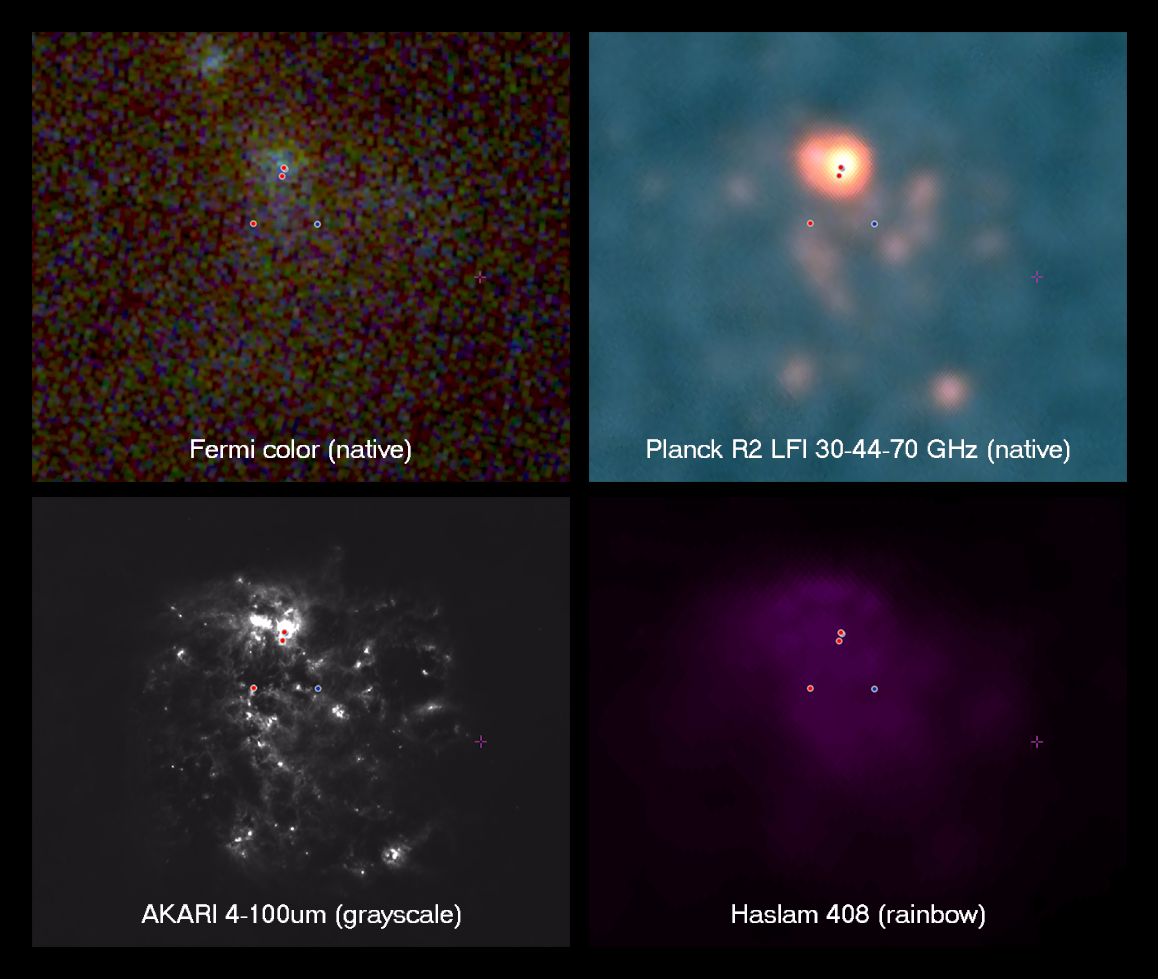
\includegraphics[width=\textwidth]{figures/lmc_region}}
%   \caption{The Large Magellanic Cloud (LMC) in various survey images and color maps, FOV 10 degrees.}
% \end{figure}

The default image layer displayed on the website's Map View page is a multi-wavelength all-sky survey from Fermi-LAT. As Fermi data is broken into multiple bands of energies, the map's native color scheme represents detected energies as categorized colors - red/yellow for the 0.3-1 GeV band, green for the 1-3 GeV band, and blue for the 3-300 GeV band.

 The Fermi color image is presented on the website as a Hierarchical Progressive Survey (HiPS) image \cite{hips}. HiPS is a hierarchical data structure utilizing the HEALPix\footnote[4]{\url{http://healpix.sourceforge.net/}} tesselation of a sphere that organizes data onto pixelated tiles of scalable resolution. The image mechanism allows catalog data and source markers on \gammasky to be visualized accurately on the sky map at various zoom levels. The Centre de Donn\'{e}es astronomiques de Strasbourg (CDS) developed the HiPS technology, and \gammasky currently encompasses 8 survey images also prepared by CDS in this format. The 8 images, which are outlined in Table~\ref{tab:images}, come from CDS's HiPS database\footnote[5]{\url{http://aladin.u-strasbg.fr/hips/list}} of over 300 prepared HiPS images.

Our website incorporates 4 source catalogs, as illustrated in Table~\ref{tab:catalogs}. 3FGL \cite{3fgl} and 2FHL \cite{2fhl} are the latest source catalogs from Fermi-LAT, the main space-based instrument we display sources from. SNRcat \cite{snrcat} is an up-to-date compilation of galactic SNRs observed from a variety of instruments. The database is maintained by the University of Manitoba and can be accessed at \url{http://www.physics.umanitoba.ca/snr/SNRcat/}. gamma-cat is an open-data catalog of sources in the TeV range. As a project that has just recently begun in early September 2016, it is undergoing rapid growth and will be updated frequently on \gammasky. gamma-cat was started at the Max-Planck-Institut f\"{u}r Kernphysik (MPIK) and is open to contribution from other developers. All of its source information can be found at \url{https://gammapy.github.io/gamma-cat/}.

User inputs for search fields under the Map View portion of the website are interpreted by the Sesame service\footnote[6]{\url{http://cds.u-strasbg.fr/cgi-bin/Sesame}}. Sesame is a search term resolver for astronomical objects which queries several databases and returns the resolved sources. Both Sesame and the databases searched (SIMBAD, NED, and VizieR) are maintained by CDS.

Under the Catalog View of \gammasky, we are currently showing 3FGL light curve and emission spectrum plots from NASA's Fermi-LAT 3FGL Catalog Interactive Table\footnote[7]{\url{http://fermi.gsfc.nasa.gov/ssc/data/access/lat/4yr_catalog/3FGL-table}}.
